% =============================================================================
% Part II, Chapter 12: Cohort 029 (CF-TP1 Confirmatory Study)
% =============================================================================
\chapter{Target-Population Transport and the Confirmatory CF-TP1 Benchmark (Cohort 029)}\label{ch:cohort_029}

Every methodological failure, shortcut discovery, and control dissociation across Cohorts~001--028 converged into the design of \textbf{Cohort~029}, governed by frozen protocol \textbf{\texttt{CF-TP1 v1.0}} (\texttt{experiments/cohort\_029/CF-TP1-v1.0.md}) and tagged as annotated release \texttt{cohort-029-v1.0.0} (\nolinkurl{76206c259caa488668a7556ce1bc53cb35d220da}). Rather than testing single-item accuracy on an unmatched causal prompt, Cohort~029 constructed a cryptographically frozen, exact-rational, $128$-family ($4{,}096$-prompt) benchmark testing \textbf{target-population causal transportability} side by side against an algebraically isomorphic \textbf{weighted-scorecard arithmetic control} on \texttt{Qwen2.5-7B-Instruct Q4\_K\_M}. Chapter~21 in Part~V presents the full mathematical construction of \texttt{CF-TP1}; here we chronicle Cohort~029 in our standard 13-part historical format and reconcile a crucial manual transcription discrepancy in its prose release summary.

% =============================================================================
\section{Cohort 029: Frozen 128-Family \texttt{CF-TP1} Target-Transport Confirmatory Case Study}

\subsection*{1. Historical Context}
By November 23, 2026, CausalFade had proved two uncomfortable truths: (1) two-study selection benchmarks without subgroup standardization admitted magnitude shortcuts (Cohort~016) or single-pass distractor interference (Cohorts~020--024), and (2) abstract $P(W,X,Y)$ graph-switch prompts yielded $0/8$ paired switching across \texttt{F16} models (Cohorts~027--028). Cohort~029 united realistic two-study provenance (randomized study vs.\ confounded historical study) with pre-treatment subgroup effect heterogeneity (\texttt{Amber} vs.\ \texttt{Blue}) and \textbf{target-population composition shifts} ($w_0$ vs.\ $w_1$), audited against $162$ deterministic noncausal shortcut policies before freezing a single byte of model inference.

\subsection*{2. Research Question}
On \texttt{Qwen2.5-7B-Instruct Q4\_K\_M} under a cryptographically frozen protocol, what is target-pair decision fidelity on natural-prose causal transport tasks versus matched weighted-scorecard arithmetic controls, and how do pairwise decision reversals and invariances decompose across the two tasks?

\subsection*{3. Hypothesis}
\textbf{Classification:} \emph{Documented prospective frozen confirmatory case study (\texttt{H15}--\texttt{H20}, \texttt{CF-TP1-v1.0.md}).} Primary pre-registered endpoint: stratified family-cluster difference $\Delta = F_{\mathrm{target,transfer}}(\text{causal}) - F_{\mathrm{target,transfer}}(\text{arithmetic})$ across $128$ independent families ($512$ transfer target pairs per task), accompanied by both Welch--Satterthwaite $t$ and finite-sample bounded 95\% confidence intervals.

\subsection*{4. Experimental Design}
\begin{itemize}
  \item \textbf{Model:} \texttt{Qwen2.5-7B-Instruct Q4\_K\_M} (\texttt{temperature=0.0}, stateless \texttt{/v1/chat/completions}). \emph{Historical note:} While \texttt{Q4\_K\_M} was practical on the local host and connected back to Cohort~016's 7B \texttt{Q4\_K\_M} focus, the specific rationale for executing Cohort~029 solely on \texttt{Qwen2.5-7B Q4\_K\_M} rather than pairing it with \texttt{F16} is not explicitly stated in \texttt{CF-TP1-v1.0.md} and is therefore recorded as \emph{undocumented beyond single-checkpoint case-study scoping}.
  \item \textbf{Factorial Structure ($4{,}096$ stateless prompts):} $128$ fresh exact-rational world families (\texttt{seed=290431}, stratified across $H=8$ blocks of $16$ families spanning the $2\times 2$ sign-matrix classes $(p,g)\in\{0,1\}^2$ and initial polarity $b\in\{-1,+1\}$) $\times 2$ wording forms (\texttt{archive}=0, \texttt{transfer}=1) $\times 2$ task domains (\texttt{causal}=0, \texttt{arithmetic}=1) $\times 2$ study display orders $\times 2$ randomized-source role assignments (\texttt{A} vs.\ \texttt{B}) $\times 2$ target population mixes ($w_0$ vs.\ $w_1$) $= 128 \times 32 = \mathbf{4{,}096}$ prompts.
  \item \textbf{Option Order:} Balanced deterministically via parity over family/design indices (\texttt{{"activate":1} or {"activate":0}} vs.\ \texttt{{"activate":0} or {"activate":1}}).
\end{itemize}

\subsection*{5. Mathematical Formulation}
For each world family $i$, randomized source $r \in \{0,1\}$, and target mix $w_m \in \{w_{i,0}, w_{i,1}\}$, both the causal transport task and the matched scorecard task share the exact rational target difference:
\begin{equation}
  \tau_{i,r}(w_m) = w_m \bigl(\mu_{i,r}(0,1) - \mu_{i,r}(0,0)\bigr) + (1 - w_m)\bigl(\mu_{i,r}(1,1) - \mu_{i,r}(1,0)\bigr) \neq 0,
\end{equation}
with optimal action $g_{i,r,m} = \mathbb{I}(\tau_{i,r}(w_m) > 0)$. Target-pair fidelity scores $1$ iff the model predicts \emph{both} target mixes $(m=0, m=1)$ correctly holding $(i, \text{form}, \text{task}, \text{order}, \text{role})$ fixed: $F = \mathbb{I}(\hat{a}_0 = g_0 \;\wedge\; \hat{a}_1 = g_1)$.

\subsection*{6. Experimental Execution}
Frozen prior to inference under manifest SHA-256 \nolinkurl{5252f69d30a0a5bb65a5efa669458e325c0531f25ab55f768531c7ca29f4c766}, with pre-run fixture and $162$-policy shortcut audits verified in \texttt{fixture\_audit.json} and \texttt{policy\_audit.json}. Confirmatory inference ran cleanly on November 25, 2026 (\texttt{08:15 UTC} onward), logging all $4{,}096$ intent, dispatch, and base64-encoded raw HTTP response records into \texttt{events.jsonl} (SHA-256 \nolinkurl{673eb723637614dc8b94875f2e8c4e9e20234c1d179c992791853797875977bd}). Strict duplicate-rejecting JSON compliance was \textbf{$4{,}096/4{,}096$ ($100.00\%$)} with zero retries or truncations.

\subsection*{7. Results}
Figure~\ref{fig:c29_final} and Table~\ref{tab:c29_reconciliation} present the complete verified confirmatory findings alongside our audit reconciliation of \texttt{RESULTS.md}.

\begin{figure}[htbp]
  \centering
  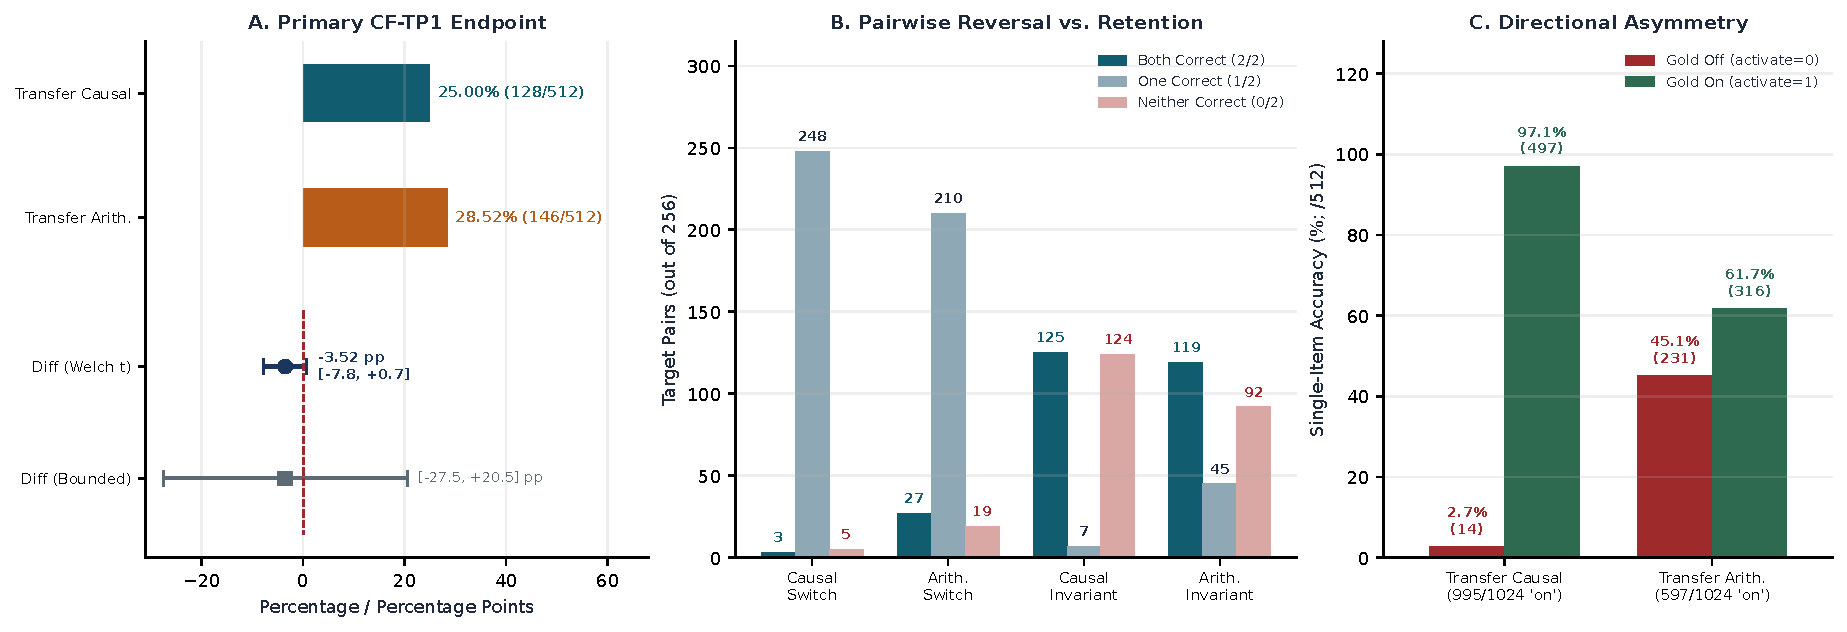
\includegraphics[width=\textwidth]{figures/fig14_cohort029_final_results.pdf}
  \caption{Cohort~029 confirmatory \texttt{CF-TP1} results on \texttt{Qwen2.5-7B-Instruct Q4\_K\_M} ($4{,}096/4{,}096$ strict-valid responses): (A) Primary transfer target-pair fidelity and paired difference intervals; (B) Pairwise correctness split by required reversal ($256$ pairs) vs.\ required invariance ($256$ pairs); (C) Single-item accuracy split by \texttt{Gold Off (0)} vs.\ \texttt{Gold On (1)}, revealing near-universal \texttt{activate=1} collapse ($995/1{,}024$) under causal framing.}
  \label{fig:c29_final}
\end{figure}

\begin{table}[htbp]
\centering
\footnotesize
\caption{Cohort 029 confirmatory metrics on \texttt{Qwen2.5-7B-Instruct Q4\_K\_M} ($4{,}096/4{,}096$ strict-valid responses) and explicit reconciliation of the manual prose transcription error in \texttt{experiments/cohort\_029/release/RESULTS.md}.}\label{tab:c29_reconciliation}
\begin{tabular}{@{}>{\raggedright\arraybackslash}p{4.8cm}>{\raggedright\arraybackslash}p{3.0cm}>{\raggedright\arraybackslash}p{3.2cm}>{\raggedright\arraybackslash}p{3.2cm}@{}}
\toprule
\textbf{Metric (Transfer Form unless noted)} & \textbf{\texttt{RESULTS.md} Prose} & \textbf{Verified Raw Journal \& \texttt{secondary.json}} & \textbf{Audit Status} \\
\midrule
Primary Causal Target-Pair Fidelity & 128/512 (25.00\%) & 128/512 (25.00\%) & Exact match \\
Primary Arithmetic Target-Pair Fidelity & 146/512 (28.52\%) & 146/512 (28.515625\%) & Exact match \\
Paired Difference $\widehat{\Delta}$ (Welch $t$ 95\% CI) & $-3.52$ pp [$-7.77, +0.74$] & $-3.515625$ pp [$-7.7713, +0.7400$] & Exact match \\
Bounded 95\% Confidence Interval & [$-27.52, +20.49$] pp & [$-27.5237, +20.4924$] pp & Exact match \\
Archive Causal / Arithmetic Fidelity & 128/512 vs.\ 128/512 & 128/512 vs.\ 128/512 ($\Delta=0$) & Exact match \\
Transfer Causal: Gold-Off (0) Correct & 121/512 (erroneous) & \textbf{14/512 (2.73\%)} & Manual prose typo \\
Transfer Causal: Gold-On (1) Correct & 416/512 (erroneous) & \textbf{497/512 (97.07\%)} & Manual prose typo \\
Transfer Causal: Total \texttt{activate=1} & 995/1024 (97.17\%) & \textbf{995/1024 (97.17\%)} & Internally inconsistent in \texttt{RESULTS.md} \\
Transfer Arith.: Gold-Off (0) Correct & 124/512 (erroneous) & \textbf{231/512 (45.12\%)} & Manual prose typo \\
Transfer Arith.: Gold-On (1) Correct & 397/512 (erroneous) & \textbf{316/512 (61.72\%)} & Manual prose typo \\
Transfer Arith.: Total \texttt{activate=1} & 785/1024 (erroneous) & \textbf{597/1024 (58.30\%)} & Manual prose typo \\
Transfer Switch Pairs: Both Correct & 3/256 (C) vs.\ 27/256 (A) & 3/256 (C) vs.\ 27/256 (A) & Exact match \\
Transfer Invariant Pairs: Both Correct & 125/256 (C) vs.\ 119/256 (A) & 125/256 (C) vs.\ 119/256 (A) & Exact match \\
\bottomrule
\end{tabular}
\end{table}

\begin{itemize}
  \item \textbf{Primary Confirmatory Endpoint (Transfer Form):}
    \begin{itemize}
      \item \textbf{Causal Target-Pair Fidelity:} \textbf{$128/512$ ($25.0000\%$)}, stratified 95\% Welch $t$ CI $[22.25\%, 27.75\%]$.
      \item \textbf{Matched Arithmetic Target-Pair Fidelity:} \textbf{$146/512$ ($28.515625\%$)}, stratified 95\% Welch $t$ CI $[24.80\%, 32.23\%]$.
      \item \textbf{Paired Causal-Minus-Arithmetic Contrast:} \textbf{$\widehat{\Delta} = -3.515625\pp$\textbf{ ($\widehat{\mathrm{SE}} = 2.1324\pp$, $\hat{\nu} = 67.53$), }95\% Welch $t$ CI $[-7.7713, +0.7400]\pp$}, finite-sample \textbf{95\% bounded CI $[-27.5237, +20.4924]\pp$\textbf{---statistically }inconclusive} (crossing zero in both intervals).
    \end{itemize}
  \item \textbf{Archive Wording Form:} Scored \textbf{$128/512$ ($25.00\%$)} on causal and \textbf{$128/512$ ($25.00\%$)} on arithmetic ($\widehat{\Delta}_{\mathrm{archive}} = 0.00\pp$).
  \item \textbf{Qualitative Behavioral Divergence Behind Similar Pairwise Totals:} Decomposing the $512$ transfer target pairs into the $256$ \textbf{reversal-required} pairs ($g_0 \neq g_1$) and $256$ \textbf{invariance-required} pairs ($g_0 = g_1$) exposed radically different failure mechanisms:
    \begin{itemize}
      \item \emph{Transfer Causal:} Output \texttt{"activate": 1} on \textbf{$995/1{,}024$ items ($97.17\%$)}! Consequently, it scored \textbf{$497/512$ ($97.07\%$)\textbf{ when \texttt{Gold=1} vs.\ }$14/512$ ($2.73\%$)} when \texttt{Gold=0} ($511/1{,}024 = 49.90\%$ item accuracy). On the $256$ target-switch pairs, it changed its action $8$ times total, achieving only \textbf{$3/256$ ($1.17\%$)} valid reversals ($248$ one-correct, $5$ wrong-way double-errors!), while scoring $125/256$ ($48.83\%$) on invariant pairs purely because roughly half of invariant pairs had $g_0=g_1=1$!
      \item \emph{Transfer Arithmetic:} Output \texttt{"activate": 1} on \textbf{$597/1{,}024$ items ($58.30\%$)}, scoring \textbf{$316/512$ ($61.72\%$)} when \texttt{Gold=1} and \textbf{$231/512$ ($45.12\%$)} when \texttt{Gold=0} ($547/1{,}024 = 53.42\%$ item accuracy). It changed actions on $46/256$ switch pairs---achieving \textbf{$27/256$ ($10.55\%$)} valid reversals ($9\times$ causal's rate, plus $19$ wrong-way flips)---but also committed \textbf{$45/256$ ($17.58\%$)} unwarranted flips on \emph{invariant} pairs ($119/256 = 46.48\%$ invariant both-correct), eroding its net pairwise advantage!
    \end{itemize}
  \item \textbf{Source-Role Pair Fidelity (Transfer Form):} Switching which study was labeled randomized (\texttt{Source A} vs.\ \texttt{Source B}) on identical tables yielded \textbf{$3/256$ ($1.17\%$)} causal switch-pair fidelity ($121/256$ invariant) vs.\ \textbf{$67/256$ ($26.17\%$)} arithmetic switch-pair fidelity ($126/256$ invariant), confirming that the model responded far more to ``designated scorecard'' pointers than to ``randomized vs.\ historical'' causal provenance tags ($3/256$)!
\end{itemize}

\begin{auditcallout}[Reconciling the Prose Typo in \texttt{experiments/cohort\_029/release/RESULTS.md}]
During Phase~I verification, byte-level reconstruction from \texttt{events.jsonl} and \texttt{row\_scores.jsonl} uncovered an internal arithmetic contradiction in lines~44--47 of the human-authored \texttt{experiments/cohort\_029/release/RESULTS.md}: that file reported transfer causal gold-off and gold-on correct counts as ``\texttt{121/512} and \texttt{416/512}'' while stating in the very same sentence that \texttt{activate=1} was chosen ``\texttt{995/1,024}'' times! Algebraically, if $416/512$ gold-on items are \texttt{1} and $512 - 121 = 391/512$ gold-off items are \texttt{1}, total activations would be $416 + 391 = 807 \neq 995$. By contrast, the machine-computed \texttt{secondary.json}, \texttt{row\_scores.jsonl}, \texttt{events.jsonl}, and \texttt{manuscript/supplement.tex} agree $100\%$: \textbf{$14/512$\textbf{ gold-off correct ($498$ false activations) and }$497/512$\textbf{ gold-on correct ($498 + 497 = 995$ activations), and for transfer arithmetic }$231/512$} gold-off correct, \textbf{$316/512$\textbf{ gold-on correct, and }$597/1{,}024$} activations ($281 + 316 = 597$). Per our non-negotiable immutability rules, \texttt{RESULTS.md} was left unmodified and reconciled transparently in Table~\ref{tab:c29_reconciliation}.
\end{auditcallout}

\subsection*{8. Interpretation at the Time}
Both \texttt{RESULTS.md} and \texttt{manuscript/article.tex} interpreted $\widehat{\Delta} = -3.52\pp$ ($[-7.77, +0.74]\pp$) with scrupulous restraint: \textbf{inconclusive primary difference, NOT equivalence and NOT selective causal deficit}, because baseline weighted-aggregation competence itself failed ($28.52\%$ arithmetic pair fidelity), while secondary transition tables revealed near-complete collapse into constant activation ($995/1{,}024$) under causal framing versus noisy partial responsiveness under scorecard framing.

\subsection*{9. Retrospective Interpretation}
Cohort~029 brought CausalFade full circle. Had Cohort~029 reported only single-item causal accuracy ($511/1{,}024 = 49.90\%$) without pairwise switch/invariance decomposition or matched arithmetic controls ($547/1{,}024 = 53.42\%$), it would have looked like an unremarkable coin flip. Instead, \texttt{CF-TP1}'s quartet design proved \emph{how} the coin flip happened: $97.2\%$ unconditional activation ($3/256$ target switches and $3/256$ provenance switches) under causal wording, contrasted with genuine partial cue responsiveness ($67/256$ scorecard switches, $27/256$ weight switches) crippled by noisy arithmetic execution ($45/256$ invariant flips) on the matched control!

\subsection*{10. Methodological Limitations}
Single confirmatory model arm (\texttt{Qwen2.5-7B-Instruct Q4\_K\_M}) without a paired Cohort~029 \texttt{F16} or frontier-model arm; stateless single-JSON output without chain-of-thought or external calculator access; two-group discrete strata; and uncertified co-author sign-off flags (\texttt{Raza} / \texttt{Umar Asghar}, \texttt{certified=false}) in pre-run blind-review metadata (examined in Chapter~18).

\subsection*{11. Scientific Contribution}
\emph{Culminating methodological benchmark (\texttt{CF-TP1}) \& rigorous diagnostic case study:} Delivered a shortcut-audited, exact-rational target-transport protocol and proved that pairwise reversal/invariance scoring separates rigid action priors from noisy aggregation failure even when aggregate accuracies nearly tie.

\subsection*{12. Transition to Subsequent Research}
Concluded empirical data collection (tagged \texttt{cohort-029-v1.0.0}) and transitioned directly into preparation of the two-part research manuscript (\texttt{manuscript/article.tex} and \texttt{supplement.tex}).

\subsection*{13. Evidence and Reproducibility}
Artifacts: \texttt{experiments/cohort\_029/CF-TP1-v1.0.md}, \texttt{freeze/manifest.json} (\texttt{5252f69d...}), \texttt{runs/confirmatory/events.jsonl} (\texttt{673eb723...}), \texttt{analysis/primary.json}, \texttt{secondary.json}, \texttt{manuscript/scripts/extract.py}; commits \texttt{76206c2}, \texttt{b737153}.
